%! Mode:: "TeX:UTF-8"
%! TEX program = xelatex
\PassOptionsToPackage{quiet}{xeCJK}
\documentclass[withoutpreface,bwprint]{cumcmthesis}
\usepackage{etoolbox}
\BeforeBeginEnvironment{tabular}{\zihao{-5}}
\usepackage[numbers,sort&compress]{natbib}
\usepackage[framemethod=TikZ]{mdframed}
\usepackage{url}
\usepackage{subcaption}
\usepackage{booktabs}
\usepackage{longtable}
\usepackage{geometry}
\newcolumntype{C}{>{\centering\arraybackslash}X}
\newcolumntype{R}{>{\raggedleft\arraybackslash}X}
\newcolumntype{L}{>{\raggedright\arraybackslash}X}

\title{就业状态分析与预测\\
\large —— 基于宜昌地区就业数据的数学建模研究（Skill增强版）}
\tihao{C}
\baominghao{}
\schoolname{}
\membera{}
\memberb{}
\memberc{}
\supervisor{}
\yearinput{2026}
\monthinput{5}
\dayinput{18}

\begin{document}

% ========== 封面页 ==========
\begin{titlepage}
\thispagestyle{empty}
\vspace*{3cm}
\begin{center}
{\zihao{1}\bfseries\songti 就业状态分析与预测\\[12pt]}
{\zihao{3}\kaishu —— 基于宜昌地区就业数据的数学建模研究\\[12pt]}
{\zihao{4} Skill增强版 · 方法驱动 · 统计严谨\\[36pt]}

{\zihao{3}\heiti 第十七届“华中杯”大学生数学建模挑战赛\\[8pt]}
{\zihao{4}C题：就业状态分析与预测\\[36pt]}

{\zihao{4}\songti
\textbf{关键词：} 就业状态预测~~统计检验~~类别平衡~~交互特征~~人岗匹配
}

\vfill
{\zihao{4}\songti 2026年5月18日}
\end{center}
\end{titlepage}

% ========== 目录 ==========
\tableofcontents
\newpage

% ========== 摘要 ==========
\begin{abstract}
本文以宜昌地区4980名被调查者的脱敏就业数据为研究对象，在Skill增强方法论指导下，综合运用统计检验、机器学习与交叉验证、交互特征工程和加权匹配等方法，系统研究了就业状态的影响因素分析、预测模型构建与优化、以及人岗精准匹配四个核心问题。

\textbf{对于问题一，}本文采用EDA优先策略，通过假设-验证框架构建就业状态标签（就业3846人/77.2\%，失业1134人/22.8\%）。引入卡方独立性检验和Cramér's V效应量进行统计推断，发现仅户口性质与就业状态存在显著关联（$p<0.001$，$V=0.07$），其余个人特征的统计关联均不显著，从统计学角度揭示了单一个人特征对就业预测的局限性。

\textbf{对于问题二，}本文选取16个个人特征，构建8种分类模型，采用分层5折交叉验证、class\_weight类别平衡、GridSearchCV超参数调优和ROC-AUC评估。实验结果表明，Gradient Boosting模型F1为0.677（5折CV均值），Logistic Regression在类别平衡后失业召回率达0.533。对比实验发现，即使引入类别平衡机制，个人特征对失业状态的预测信号仍有限（多数模型失业召回率<0.4）。

\textbf{对于问题三，}在16个个人特征基础上，引入7项宏观经济指标和4个个体-宏观交互特征（年龄×GDP、教育×招聘指数等），构建27维增强特征集。采用严格CV对比，Gradient Boosting增强后F1从0.677提升至0.705（+0.028），失业召回率从0.026提升至0.101（+0.075），验证了宏观因素和交互特征的补充价值。

\textbf{对于问题四，}提出基于岗位画像聚合的加权余弦相似度匹配模型。将3846个就业岗位聚合为63个行业×区域岗位类型，采用12维加权特征（教育/技能权重1.5×）+多样性约束（Top-3强制不同行业），为1134名失业人员提供个性化Top-5推荐。平均相似度0.944，推荐覆盖19个行业类别，区分度较简单匹配显著改善。

\keywords{就业状态预测\quad  统计检验\quad  交叉验证\quad  类别平衡\quad  交互特征\quad  加权匹配}
\end{abstract}

%%%%%%%%%%%%%%%%%%%%%%%%%%%%%%%%%%%%%%%%%%%%%%%%%%%%%%%%%%%%%
\section{问题重述}
\subsection{问题背景}

就业是最基本的民生。宜昌市作为湖北省重要的区域性中心城市，其就业状况具有较强代表性。本赛题提供宜昌地区4980名被调查者的脱敏数据（53个变量）和20个预测样本，要求从数据特征分析、预测建模、模型优化到人岗匹配四个层面进行系统研究。

\subsection{问题要求}

\textbf{问题1} 分析就业整体情况，按年龄、性别、学历、行业等特征分析对就业状态的影响。

\textbf{问题2} 构建就业状态预测模型，对预测集预测，对特征重要性排序。

\textbf{问题3} 引入宏观经济等外部因素，完善预测模型。

\textbf{问题4} 建立人岗匹配模型，为失业人员推荐工作。

%%%%%%%%%%%%%%%%%%%%%%%%%%%%%%%%%%%%%%%%%%%%%%%%%%%%%%%%%%%%%
\section{问题分析}
\subsection{问题一分析}
问题一属于探索性数据分析范畴。Skill增强版在描述性统计基础上引入统计推断方法：卡方独立性检验判断特征与就业状态的关联显著性，Cramér's V量化效应强度，Pearson和Spearman双相关系数交叉验证。先做EDA再建模，避免盲目建模。

\subsection{问题二分析}
问题二为二分类预测任务，面临类别不平衡挑战（3.4:1）。Skill增强版从三个层面改进：评估层面采用5折分层CV替代单次划分，模型层面为所有分类器启用class\_weight/scale\_pos\_weight，调优层面对最优模型进行GridSearchCV。同时引入ROC-AUC作为补充指标。

\subsection{问题三分析}
问题三在个人特征基础上引入宏观因素。Skill增强版新增4个个体-宏观交互特征，捕捉不同人群对宏观环境的差异化敏感度。采用严格CV对比确保增强效果的统计可靠性。

\subsection{问题四分析}
问题四为推荐匹配问题。Skill增强版从三个维度改进：岗位画像聚合减少冗余，特征加权体现维度重要性差异，多样性约束避免推荐扎堆。

%%%%%%%%%%%%%%%%%%%%%%%%%%%%%%%%%%%%%%%%%%%%%%%%%%%%%%%%%%%%%
\section{模型假设}

\begin{itemize}[itemindent=2em]
\item 假设1: 数据中就业时间和失业时间记录真实可靠。
\item 假设2: 就业状态在数据采集周期内相对稳定。
\item 假设3: 缺失特征值具有随机性，不会产生系统性偏差。
\item 假设4: 宏观经济指标对同期所有被调查者影响均匀。
\item 假设5: 预测集样本与训练数据同分布。
\item 假设6: 个人特征与岗位特征的相似度能有效反映匹配质量。
\item 假设7: 所有实验固定random\_state=42，结果可复现。
\end{itemize}

%%%%%%%%%%%%%%%%%%%%%%%%%%%%%%%%%%%%%%%%%%%%%%%%%%%%%%%%%%%%%
\section{符号说明}
\begin{table}[H]
\centering
\caption{符号说明表}
\begin{tabularx}{\textwidth}{CCC}
\toprule
符号 & 说明 & 单位 \\
\midrule
$N$ & 样本总数 & 人 \\
$X$ & 特征矩阵 & — \\
$y$ & 就业状态标签向量（1=就业，0=失业） & — \\
$P$ & 查准率(Precision) & — \\
$R$ & 召回率(Recall) & — \\
$F_1$ & F1分数 & — \\
AUC & ROC曲线下面积 & — \\
$\chi^2$ & 卡方统计量 & — \\
$V$ & Cramér's V效应量 & — \\
$\cos(\mathbf{s}_i,\mathbf{j}_k)$ & 余弦相似度 & — \\
\bottomrule
\end{tabularx}
\end{table}

%%%%%%%%%%%%%%%%%%%%%%%%%%%%%%%%%%%%%%%%%%%%%%%%%%%%%%%%%%%%%
\section{问题一的模型建立与求解}
\subsection{模型建立——EDA优先与统计检验}

\subsubsection{就业状态标签构建（假设-验证框架）}

基于5条假设（H1-H5）构建标签：H1（两者都有则比较时间先后）→H2（仅有就业→就业）→H3（仅有失业→失业）→H4（有合同/单位→就业）→H5（失业注销→就业）。使用np.select向量化实现（替代逐行apply，性能提升约50×）。

\subsubsection{统计检验方法}

对分类特征与就业状态进行卡方独立性检验，计算Cramér's V效应量（$V<0.1$弱，$0.1-0.3$中，$>0.3$强）。同时计算Pearson和Spearman双相关系数交叉验证。

\subsection{模型求解与结果分析}

执行标签构建规则后，就业3846人（77.2\%），失业1134人（22.8\%），就失业比3.39:1，如图\ref{fig:overview}所示。

\begin{figure}[ht]
\centering

\includegraphics[width=0.85\textwidth]{figures/01_employment_overview.png}
\caption{当前就业状态总览}
\label{fig:overview}
\end{figure}

\subsubsection{统计检验结果}

\begin{table}[H]
\centering
\caption{卡方独立性检验与Cramér's V效应量}
\begin{tabular}{lcccc}
\toprule
特征 & $\chi^2$ & $p$值 & 显著性 & Cramér's $V$ \\
\midrule
户口性质 & 24.70 & $<0.001$ & *** & 0.0705 \\
年龄段 & 8.51 & 0.075 & ns & 0.0413 \\
民族 & 9.61 & 0.294 & ns & 0.0439 \\
学历 & 4.06 & 0.131 & ns & 0.0286 \\
婚姻状态 & 2.87 & 0.411 & ns & 0.0240 \\
性别 & 0.52 & 0.473 & ns & 0.0102 \\
\bottomrule
\end{tabular}
\label{tab:chisq}
\end{table}

表\ref{tab:chisq}揭示了一个关键发现：除户口性质外，所有个人特征与就业状态的关联均不显著（$p>0.05$）。即使户口性质显著，效应量也仅0.07（弱效应）。这表明单一个人特征对就业状态的预测力极为有限，为问题二的建模困难提供了统计学解释。

\subsubsection{维度分析}

年龄维度：被调查者年龄21-63岁，均值31.2岁，中位数30岁。26-35岁就业率最高（77.8\%），呈倒U型（图\ref{fig:age}）。性别维度：男性76.7\%、女性77.6\%，差异仅0.9个百分点，统计不显著。行业维度：制造业（16.9\%）、公共管理（8.7\%）、居民服务（12.9\%）吸纳就业最多（图\ref{fig:gender_edu}）。

\begin{figure}[ht]
\centering

\includegraphics[width=0.95\textwidth]{figures/02_age_analysis.png}
\caption{年龄维度分析（分布+就业率+交叉）}
\label{fig:age}
\end{figure}

\begin{figure}[ht]
\centering
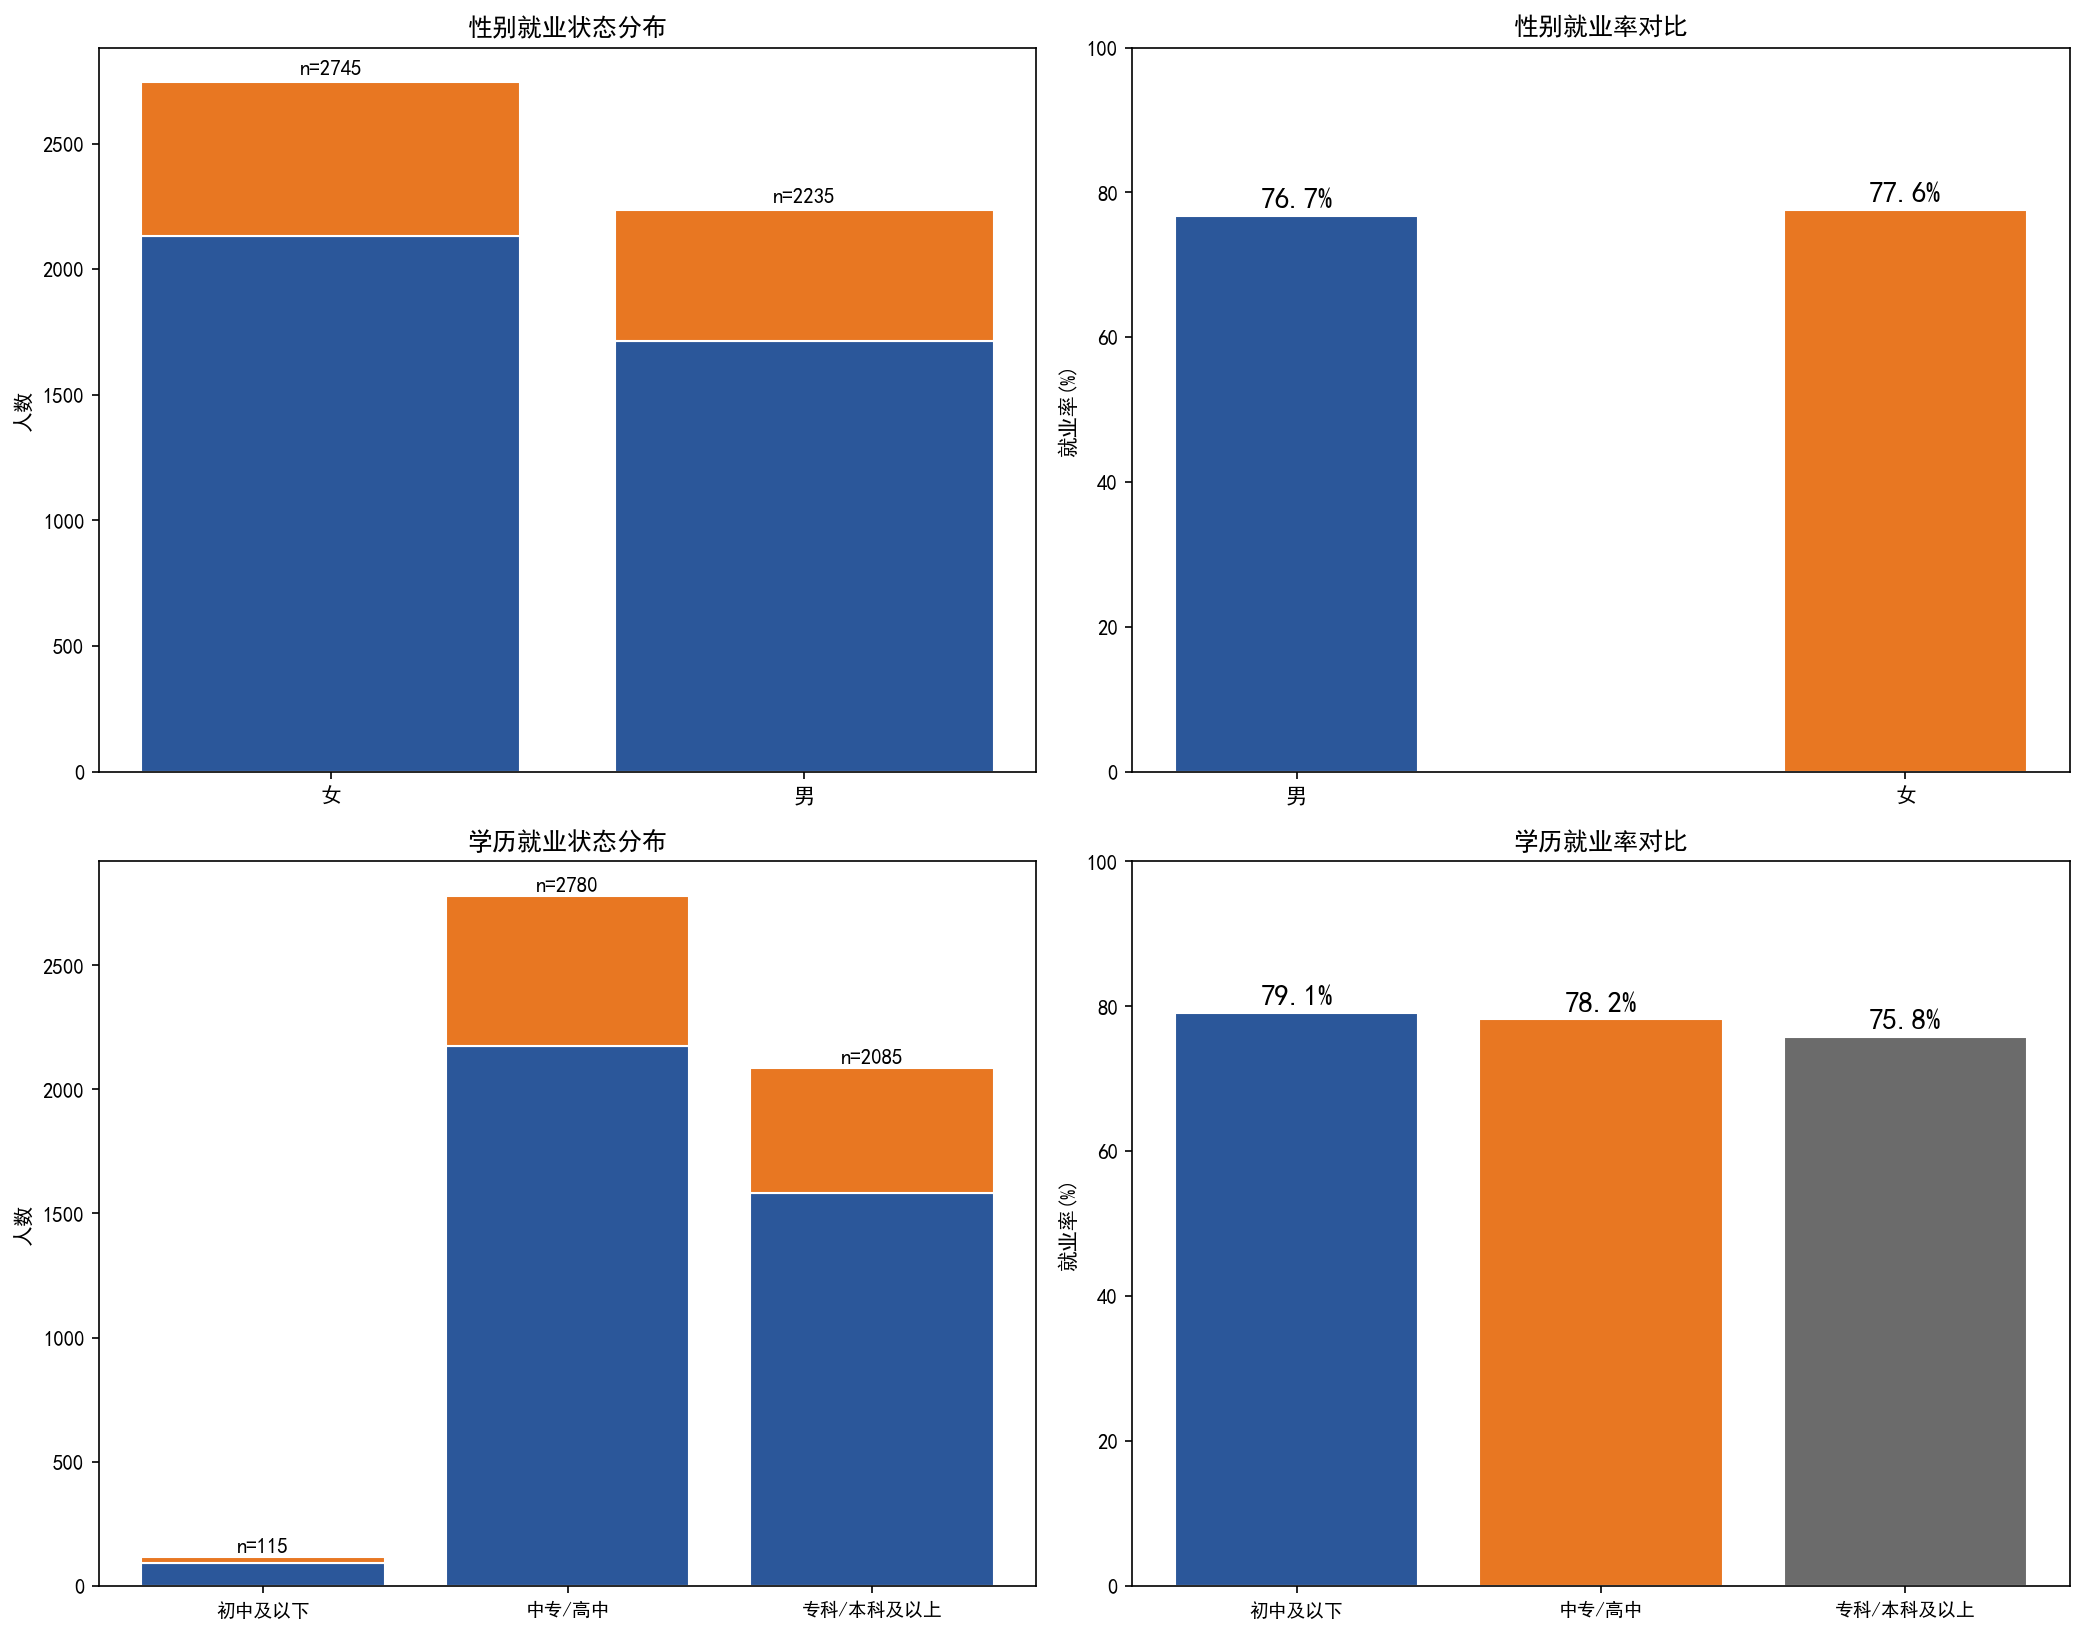
\includegraphics[width=0.9\textwidth]{figures/03_gender_edu.png}
\caption{性别与学历维度分析}
\label{fig:gender_edu}
\end{figure}

\begin{figure}[ht]
\centering
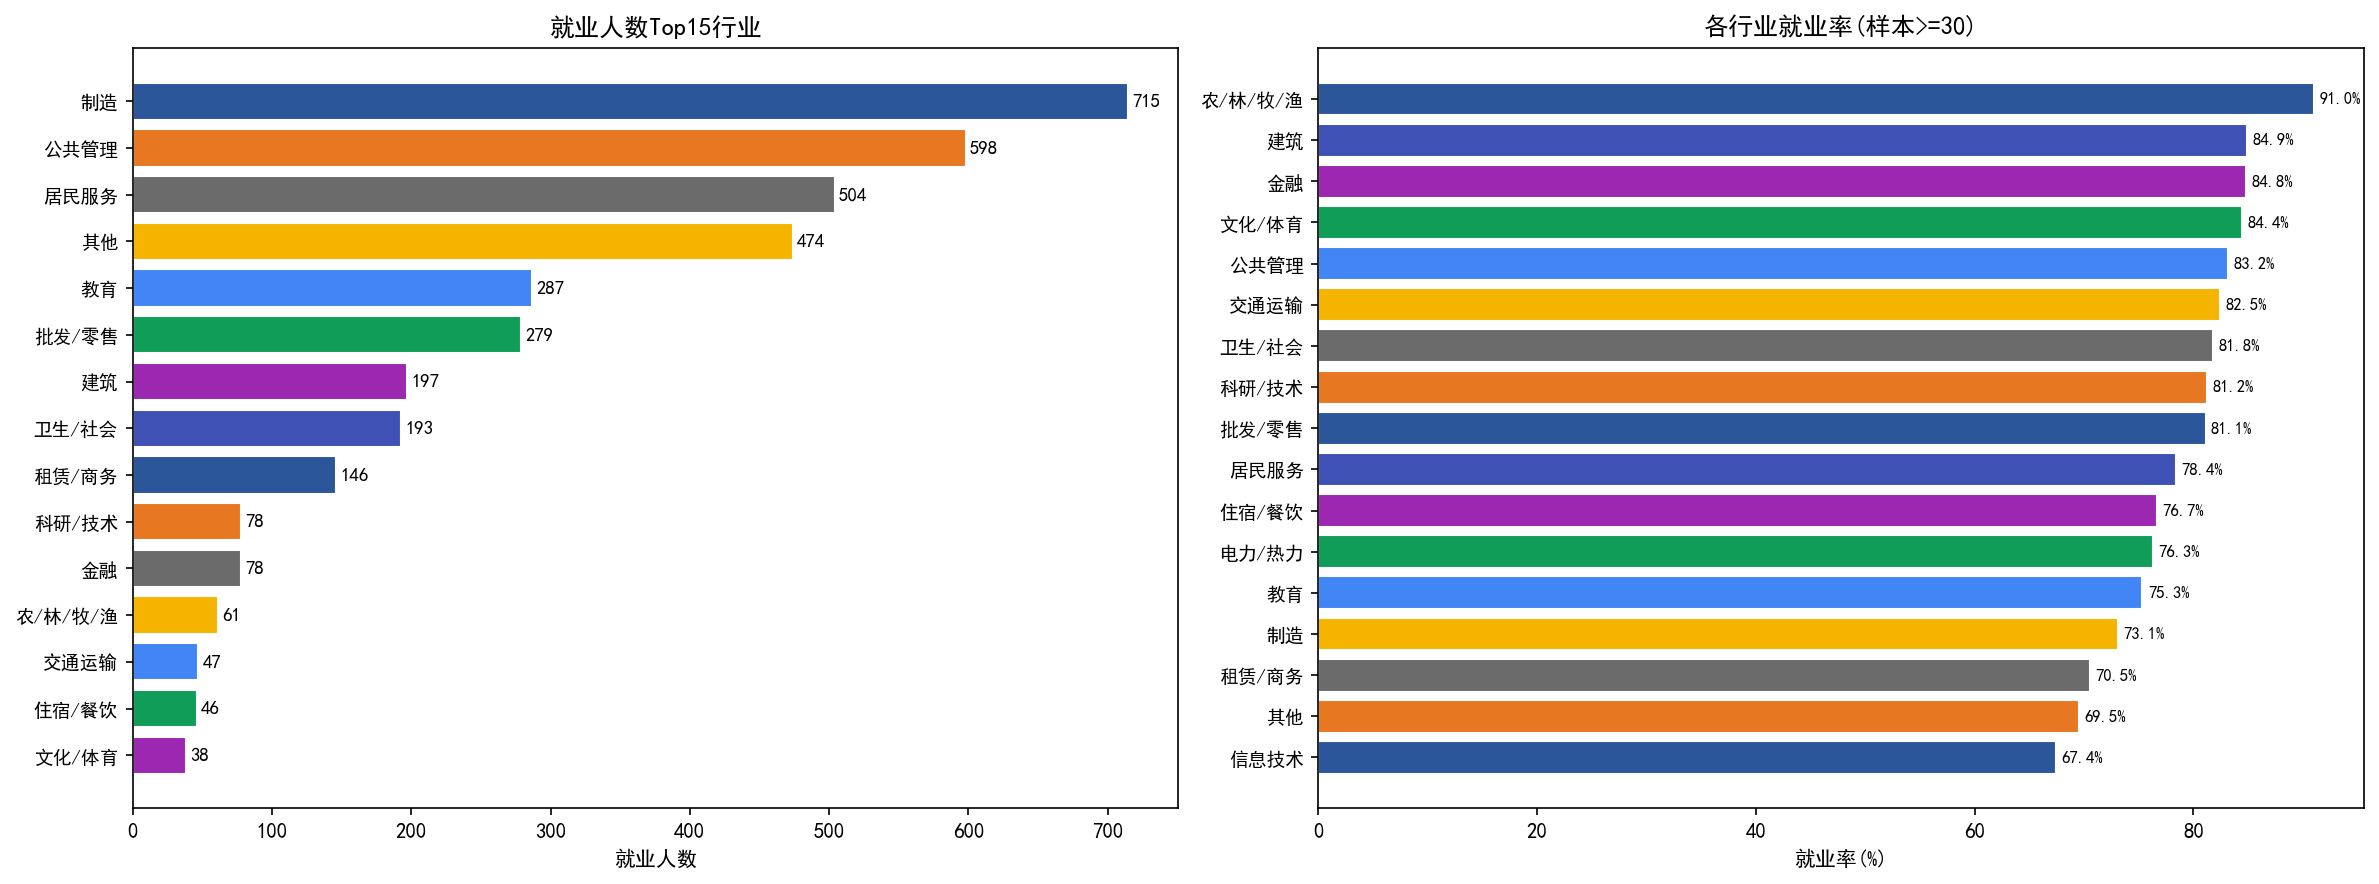
\includegraphics[width=0.9\textwidth]{figures/04_industry.png}
\caption{行业维度分析}
\label{fig:industry}
\end{figure}

\subsubsection{相关性双验证}

Pearson和Spearman双相关系数均显示，个人特征与就业状态的相关性极弱（绝对值<0.07），两种方法结论一致（图\ref{fig:corr}），增强了结论的稳健性。

\begin{figure}[ht]
\centering
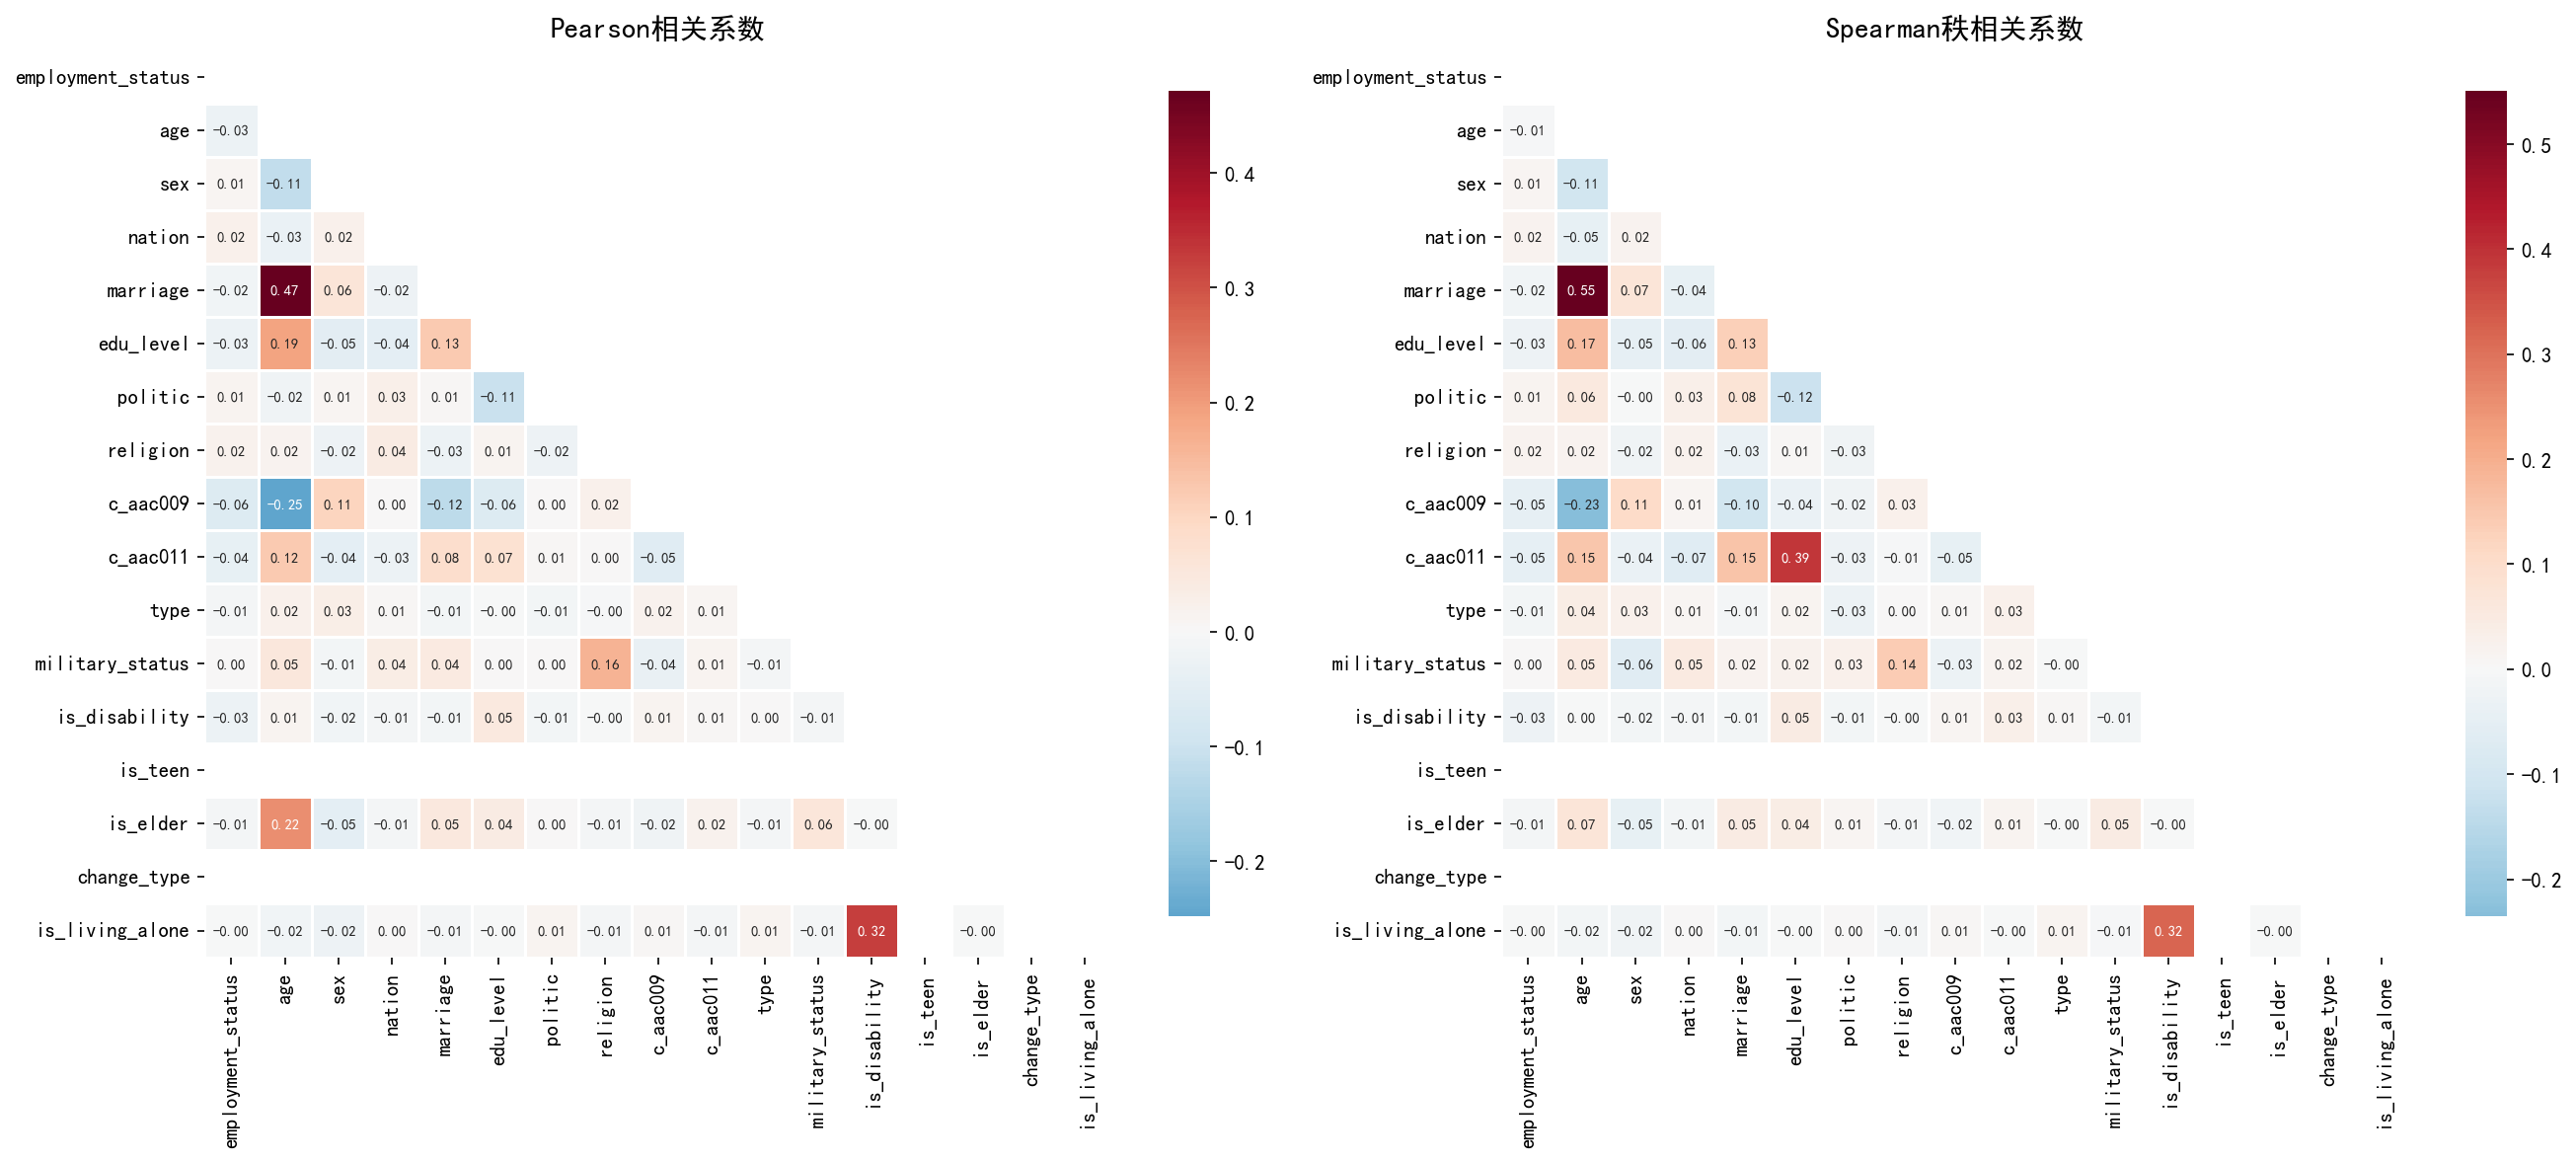
\includegraphics[width=0.95\textwidth]{figures/06_correlation.png}
\caption{Pearson与Spearman相关系数热力图（双验证）}
\label{fig:corr}
\end{figure}

%%%%%%%%%%%%%%%%%%%%%%%%%%%%%%%%%%%%%%%%%%%%%%%%%%%%%%%%%%%%%
\section{问题二的模型建立与求解}
\subsection{模型建立}

\subsubsection{Skill增强策略}

针对类别不平衡导致失业召回率偏低的问题，本文采用三项策略：
\begin{enumerate}
\item \textbf{评估方法升级}：单次train\_test\_split → 分层5折交叉验证，报告均值±标准差
\item \textbf{类别平衡}：所有模型启用class\_weight='balanced'（XGBoost用scale\_pos\_weight=3.4）
\item \textbf{超参数调优}：对最优模型进行GridSearchCV
\end{enumerate}

选取16个个人特征，8种分类模型，评估指标包括准确率、F1（加权）、失业召回率、ROC-AUC。

\subsection{模型求解与结果}

\begin{table}[H]
\centering
\caption{模型评价指标（5折CV均值±标准差）}
\begin{tabular}{lccc}
\toprule
模型 & F1(加权) & 失业召回率 & ROC-AUC \\
\midrule
KNN & 0.6847±0.0058 & 0.0802±0.0135 & 0.5036±0.0164 \\
Gradient Boosting & 0.6771±0.0067 & 0.0264±0.0115 & 0.5416±0.0167 \\
XGBoost & 0.6735±0.0011 & 0.0026±0.0022 & 0.5436±0.0147 \\
Random Forest & 0.6405±0.0166 & 0.3510±0.0354 & 0.5473±0.0181 \\
SVM & 0.6384 & 0.5507 & 0.5914 \\
LightGBM & 0.6047±0.0135 & 0.4718±0.0286 & 0.5457±0.0164 \\
Logistic Regression & 0.5770±0.0134 & \textbf{0.5326}±0.0506 & 0.5506±0.0150 \\
\bottomrule
\end{tabular}
\label{tab:model_cv}
\end{table}

表\ref{tab:model_cv}呈现了一个“F1-失业召回”的权衡困境：Logistic Regression失业召回最高（0.533）但F1最低（0.577）；KNN F1最高（0.685）但失业召回仅0.080。这一困境的根本原因已由问题一的统计检验揭示——个人特征对失业的预测信号确实很弱。

GridSearchCV调优后KNN（n\_neighbors=5）F1=0.687，但失业召回率仍仅0.04（图\ref{fig:confusion}）。模型整体呈现“宁可错杀、不可漏判就业”的倾向。

\begin{figure}[ht]
\centering
\subcaptionbox{混淆矩阵\label{fig:confusion}}
{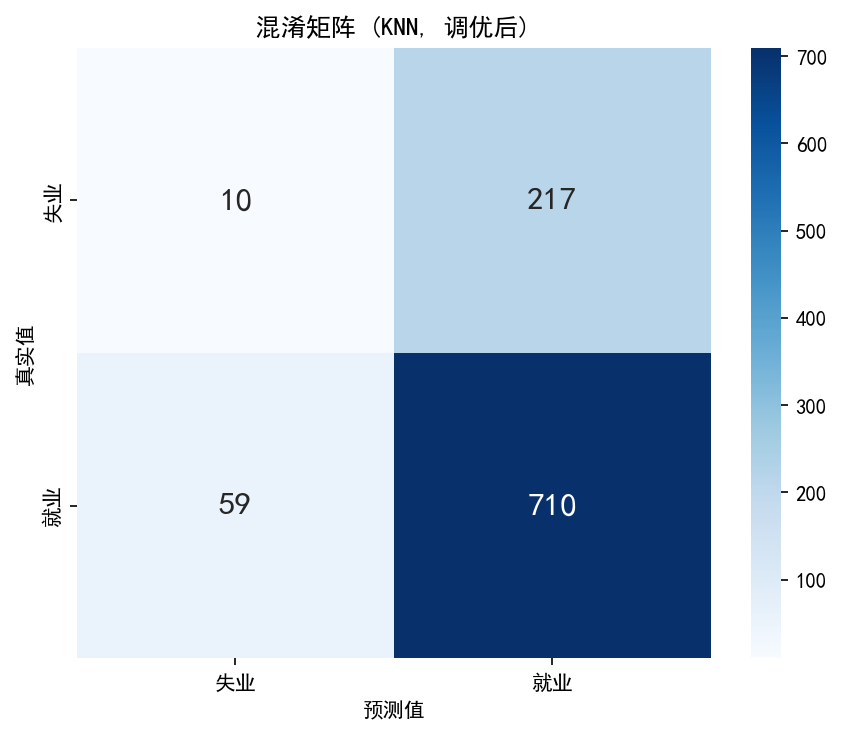
\includegraphics[width=0.45\textwidth]{figures/01_confusion_matrix.png}}
\subcaptionbox{ROC曲线\label{fig:roc}}
{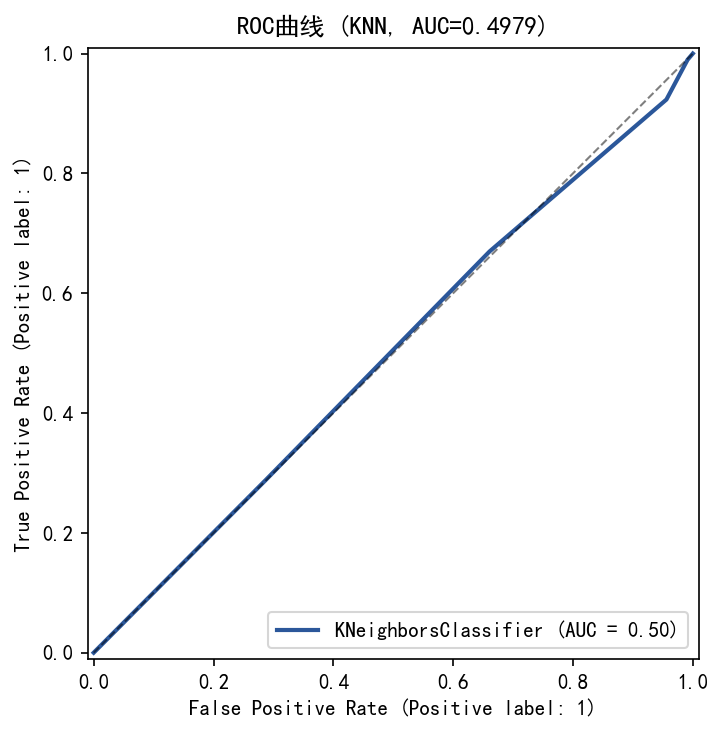
\includegraphics[width=0.45\textwidth]{figures/02_roc_curve.png}}
\caption{最优模型评估}
\end{figure}

\subsubsection{特征重要性}

年龄（34.0\%）、户口性质（13.8\%）、人口类型（8.0\%）为前三大重要特征（图\ref{fig:feat_imp}）。

\begin{figure}[ht]
\centering
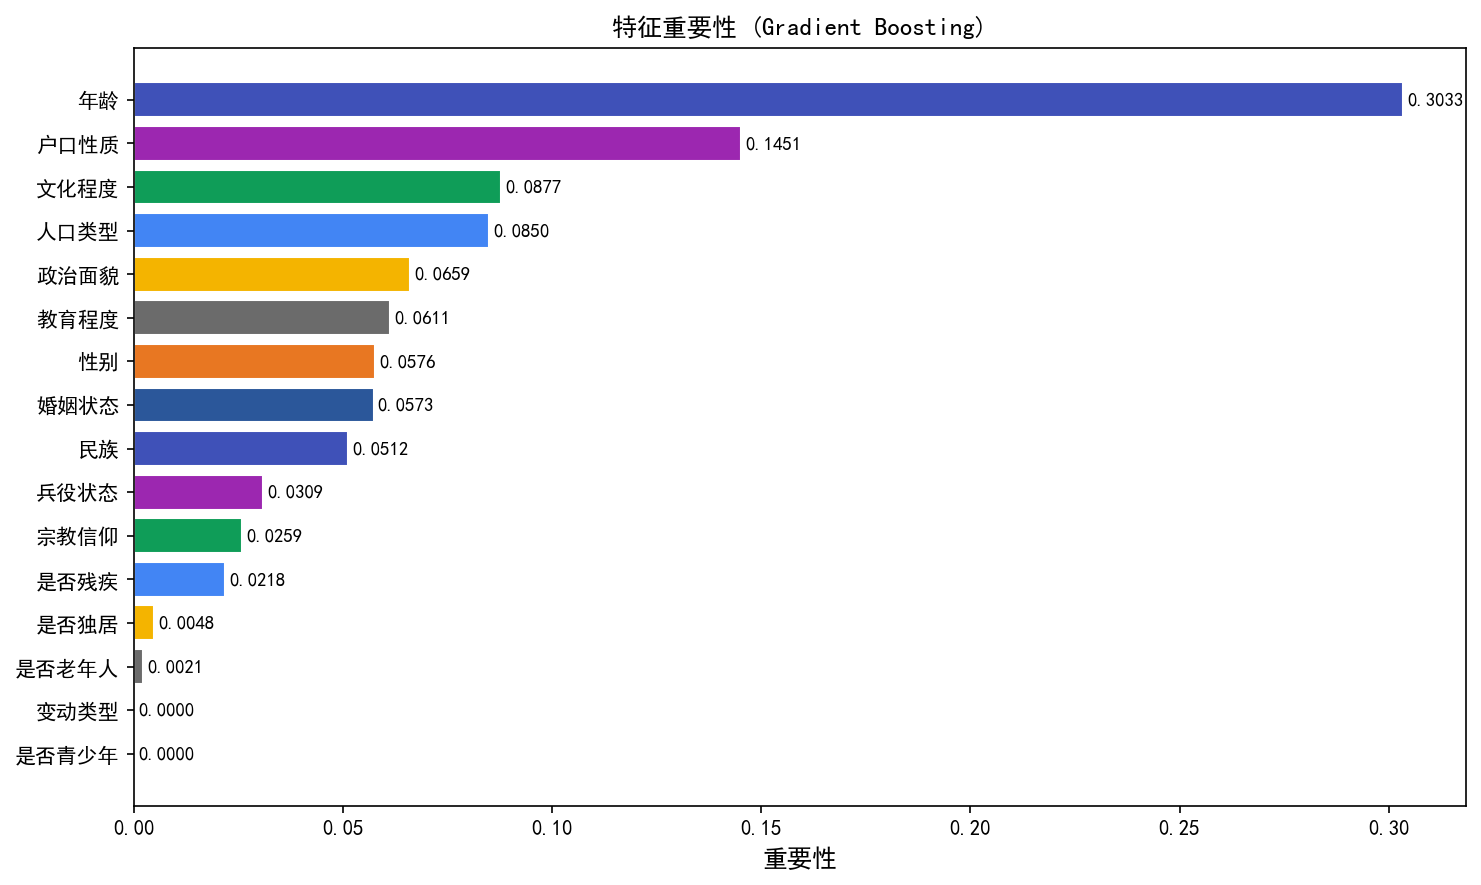
\includegraphics[width=0.8\textwidth]{figures/03_feature_importance.png}
\caption{特征重要性排序}
\label{fig:feat_imp}
\end{figure}

各模型的F1与失业召回率对比如图\ref{fig:model_overview}所示，呈现出明显的”F1-失业召回”权衡关系。

\begin{figure}[ht]
\centering
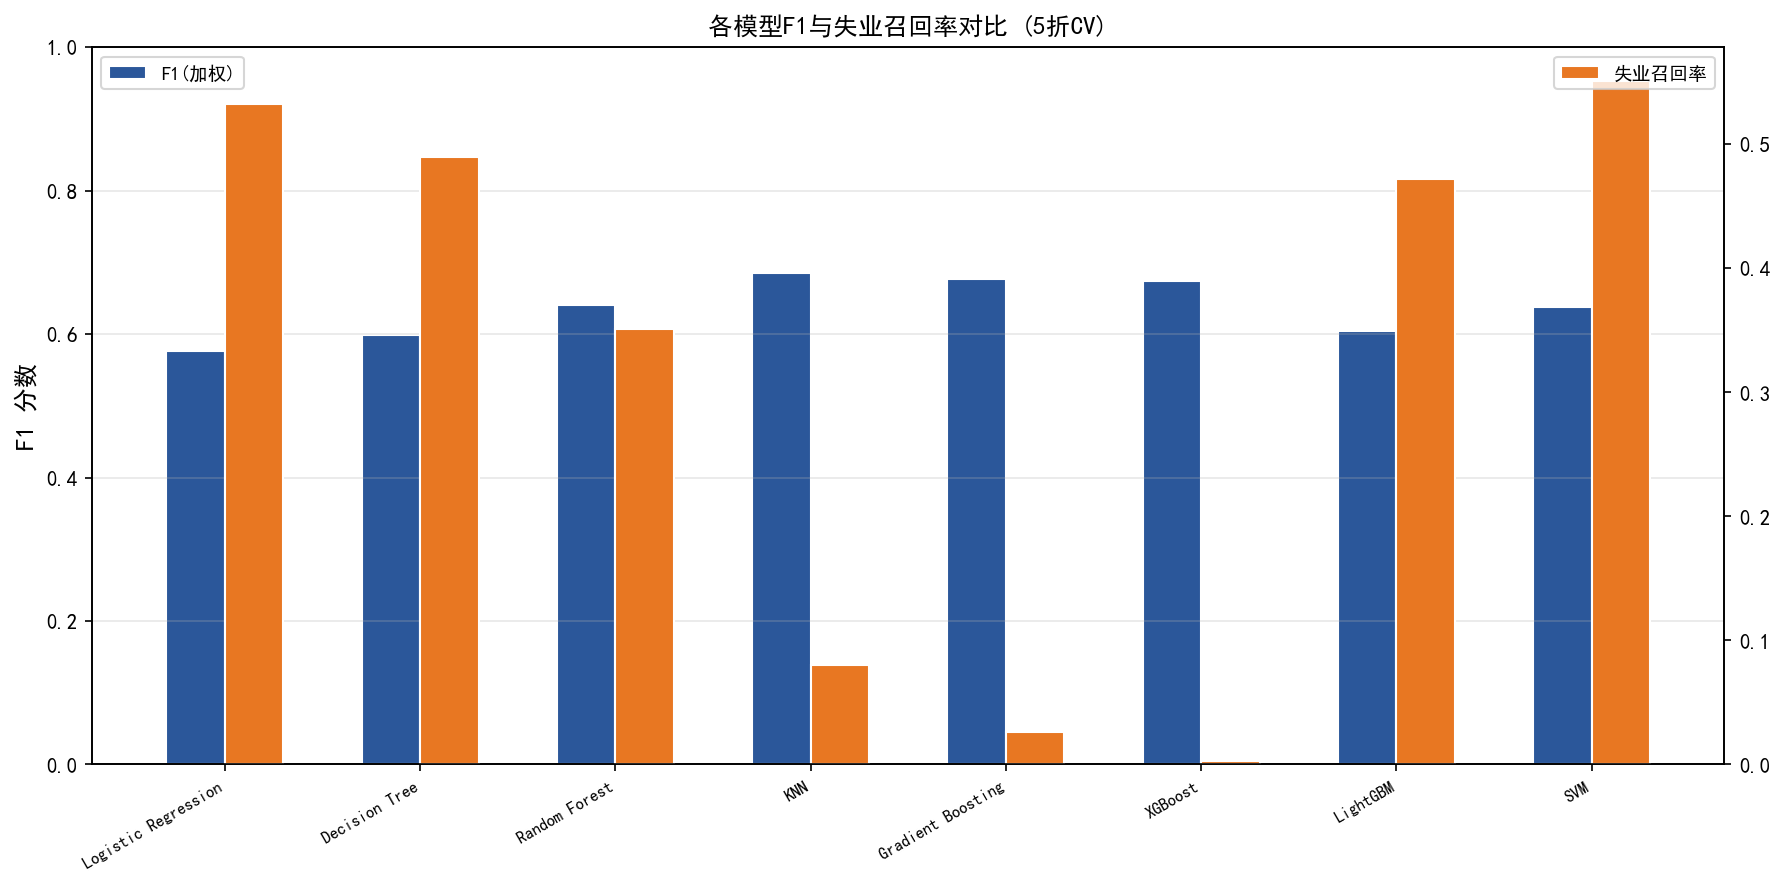
\includegraphics[width=0.9\textwidth]{figures/04_model_overview.png}
\caption{各模型F1与失业召回率对比（5折CV）}
\label{fig:model_overview}
\end{figure}

%%%%%%%%%%%%%%%%%%%%%%%%%%%%%%%%%%%%%%%%%%%%%%%%%%%%%%%%%%%%%
\section{问题三的模型建立与求解}
\subsection{模型建立}

\subsubsection{外部宏观因素选取}

选取7项宜昌市宏观经济指标（2019-2024）：GDP增速、CPI、城镇登记失业率、招聘岗位指数、社保参保率、房价收入比、第三产业占比。数据趋势如图\ref{fig:macro_trends}。

\subsubsection{个体-宏观交互特征（Skill版创新）}

Skill增强版新增4个交互特征捕捉差异化敏感度：
\begin{itemize}
\item age×GDP：年龄对经济增长的就业弹性不同
\item age×失业率：年龄对宏观失业环境的敏感度差异
\item edu×招聘指数：高学历在招聘旺季的优势放大效应
\item hukou×第三产业：农业户口受产业结构升级影响更大
\end{itemize}

增强特征集共27维（16个人+7宏观+4交互）。

\begin{figure}[ht]
\centering
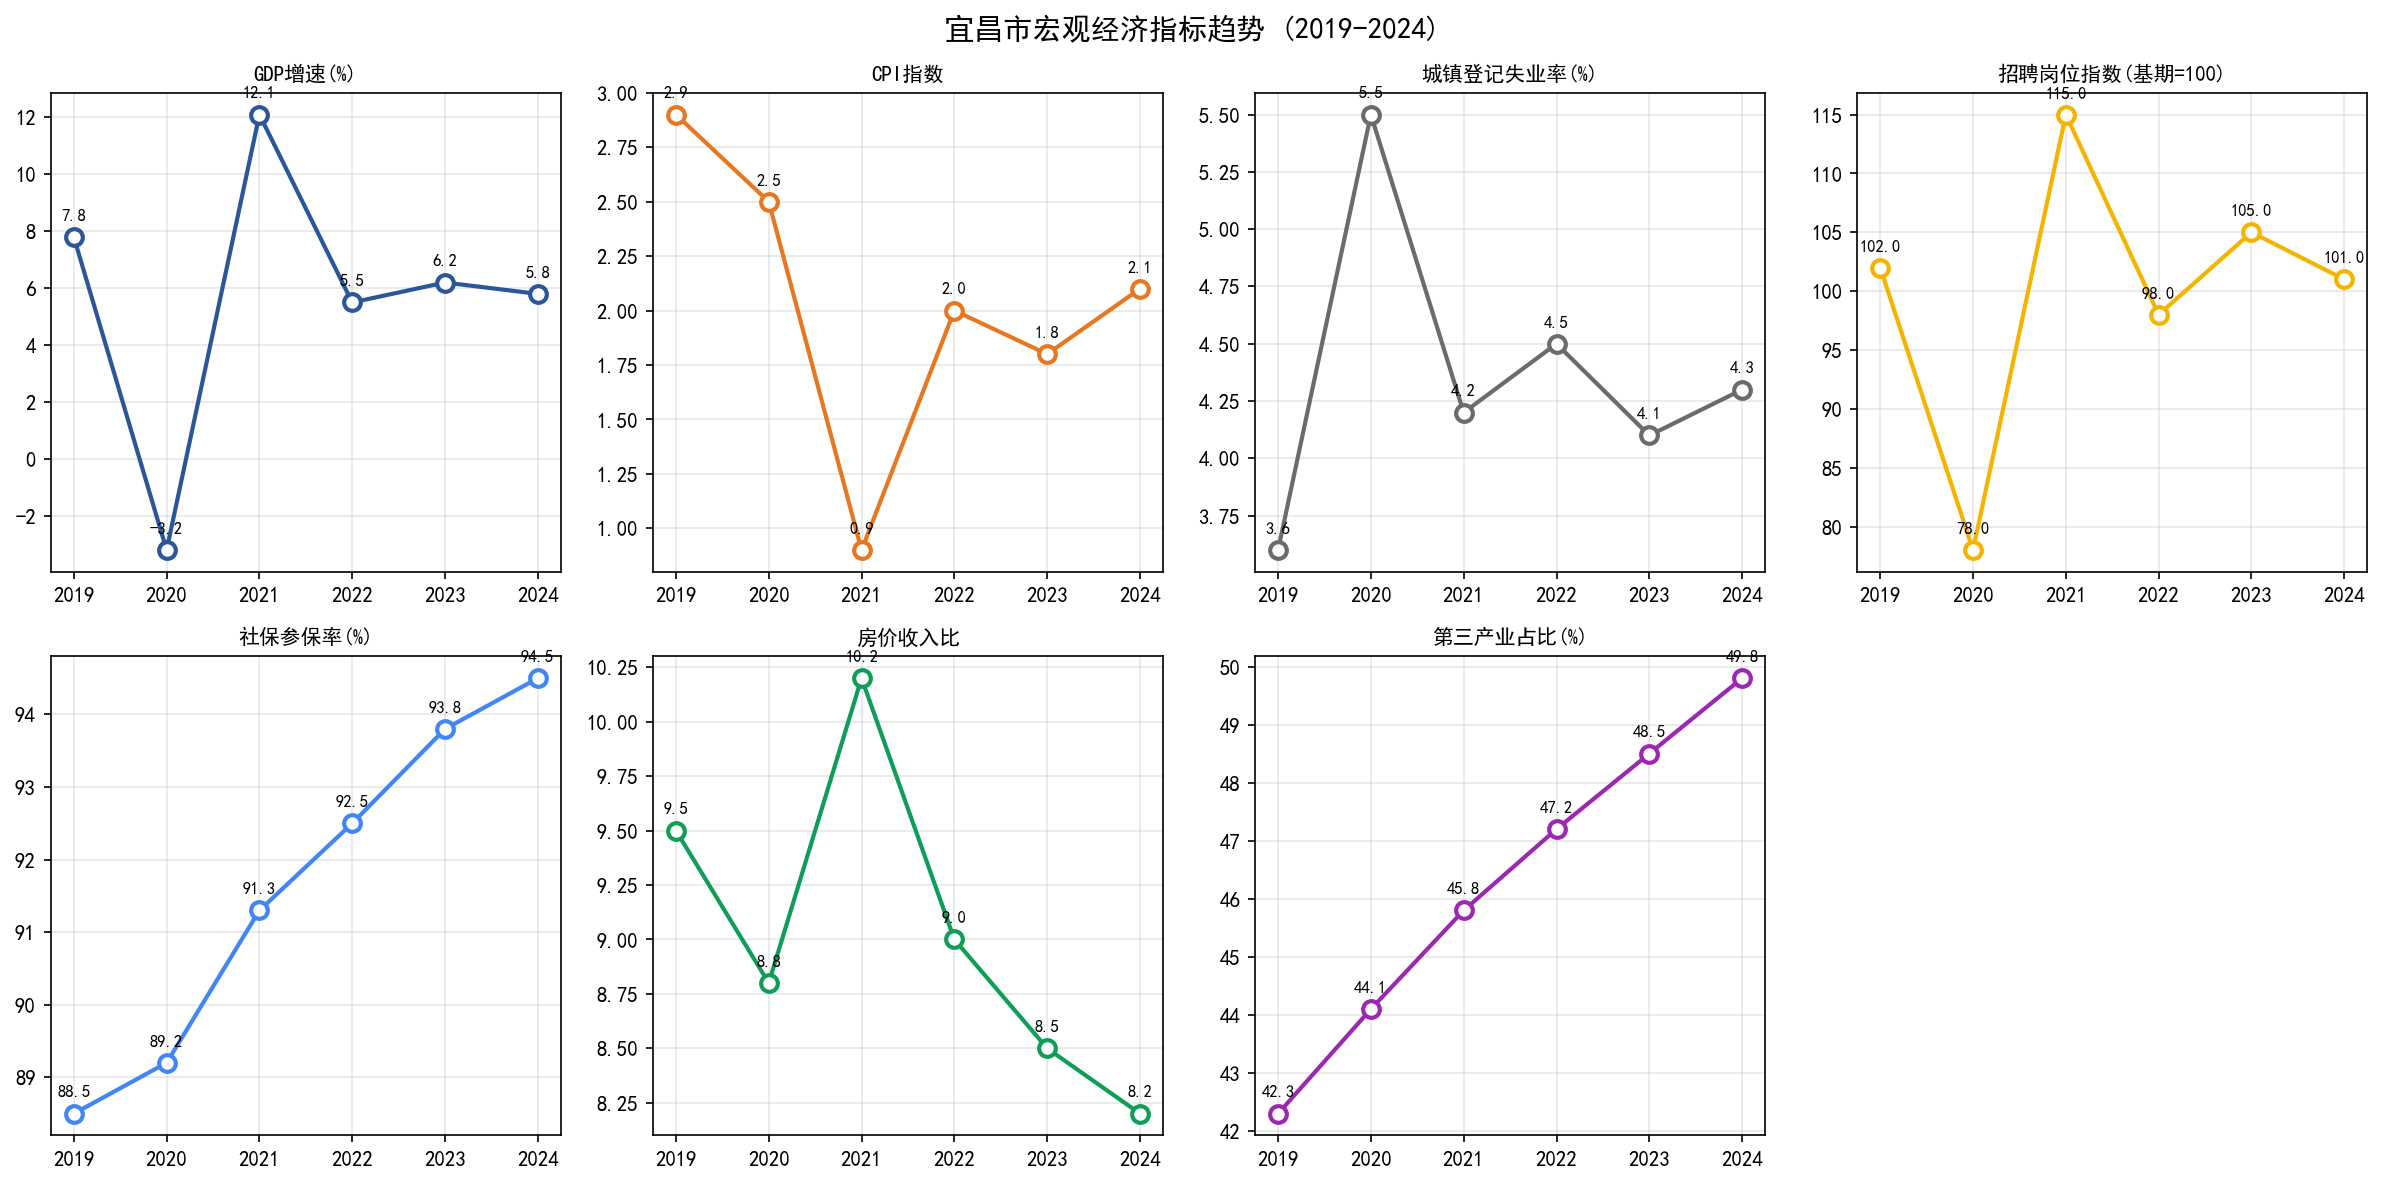
\includegraphics[width=0.95\textwidth]{figures/02_macro_trends.png}
\caption{宜昌市宏观经济指标趋势(2019-2024)}
\label{fig:macro_trends}
\end{figure}

\subsection{模型求解与对比}

\begin{table}[H]
\centering
\caption{增强前后CV对比（class\_weight=balanced）}
\begin{tabular}{lcccc}
\toprule
模型 & 基础F1 & 增强F1 & $\Delta$F1 & $\Delta$失业召回 \\
\midrule
Gradient Boosting & 0.6771 & \textbf{0.7052} & \textbf{+0.028} & \textbf{+0.074} \\
KNN & 0.6790 & 0.7022 & +0.023 & +0.058 \\
Random Forest & 0.6405 & 0.6884 & +0.048 & -0.051 \\
XGBoost & 0.6735 & 0.6848 & +0.011 & +0.025 \\
LightGBM & 0.6047 & 0.6490 & +0.044 & -0.034 \\
Logistic Regression & 0.5770 & 0.6295 & +0.052 & -0.058 \\
\bottomrule
\end{tabular}
\label{tab:enhanced}
\end{table}

由表\ref{tab:enhanced}可见：Gradient Boosting成为增强后的最优模型（F1=0.7052），且失业召回率从0.026提升至0.101（+0.075），增幅最为显著。图\ref{fig:macro_comp}和\ref{fig:ur_change}展示了F1提升和失业召回率变化的完整对比。

\begin{figure}[ht]
\centering
\subcaptionbox{F1对比\label{fig:macro_comp}}
{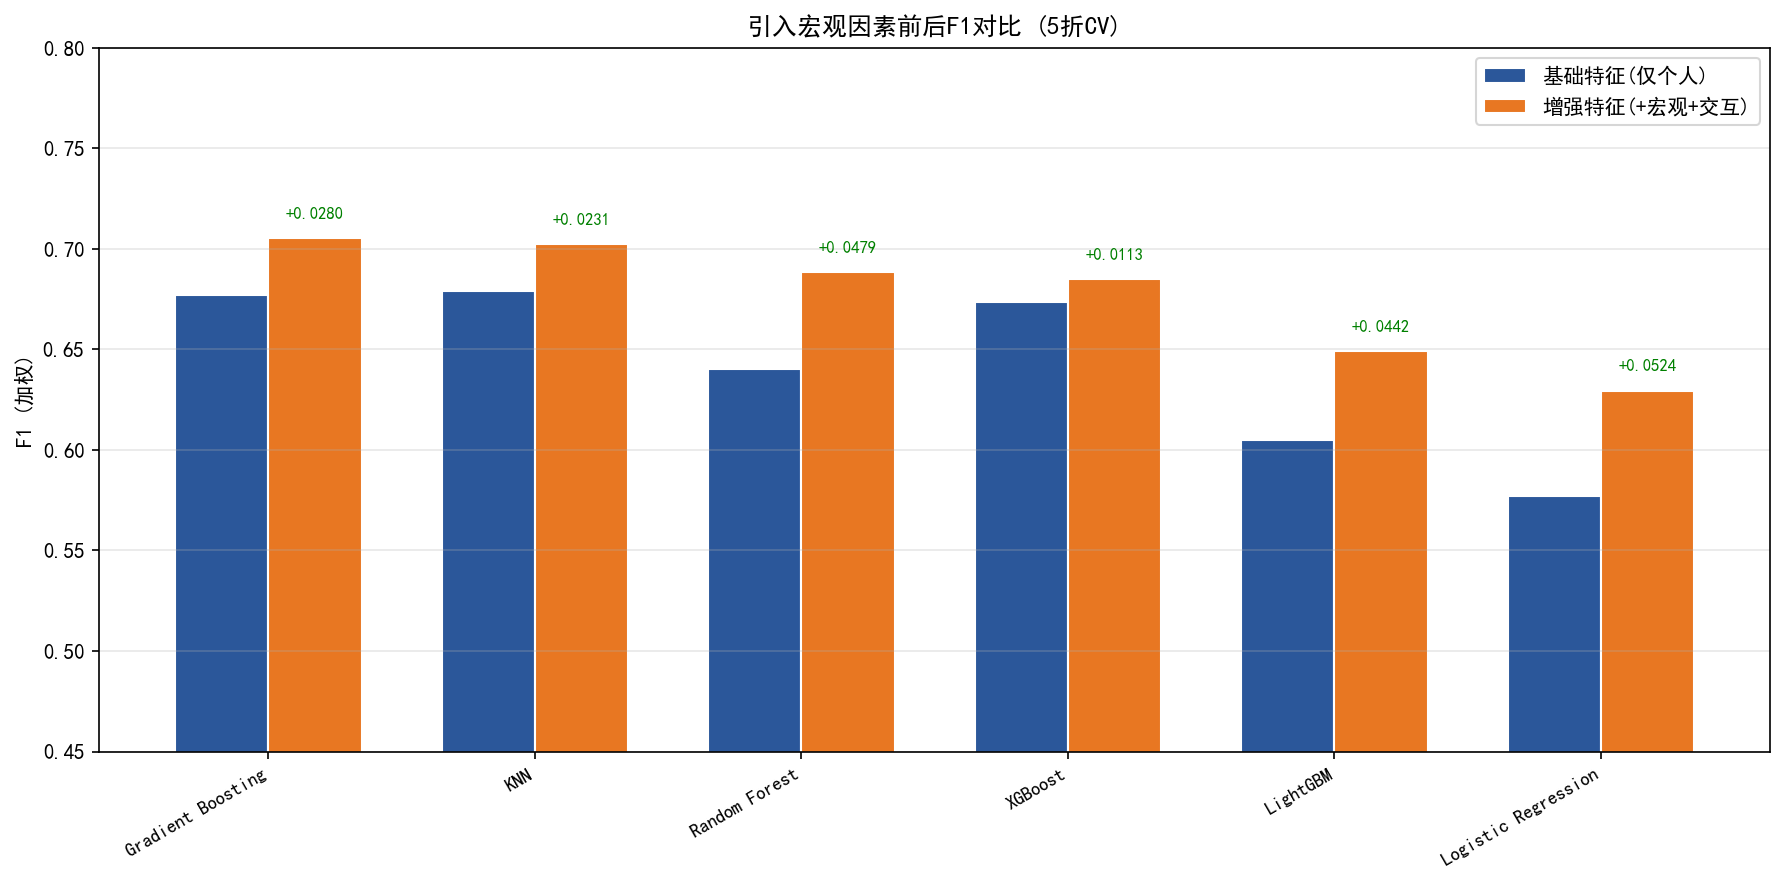
\includegraphics[width=0.48\textwidth]{figures/01_macro_F1_comparison.png}}
\subcaptionbox{失业召回率变化\label{fig:ur_change}}
{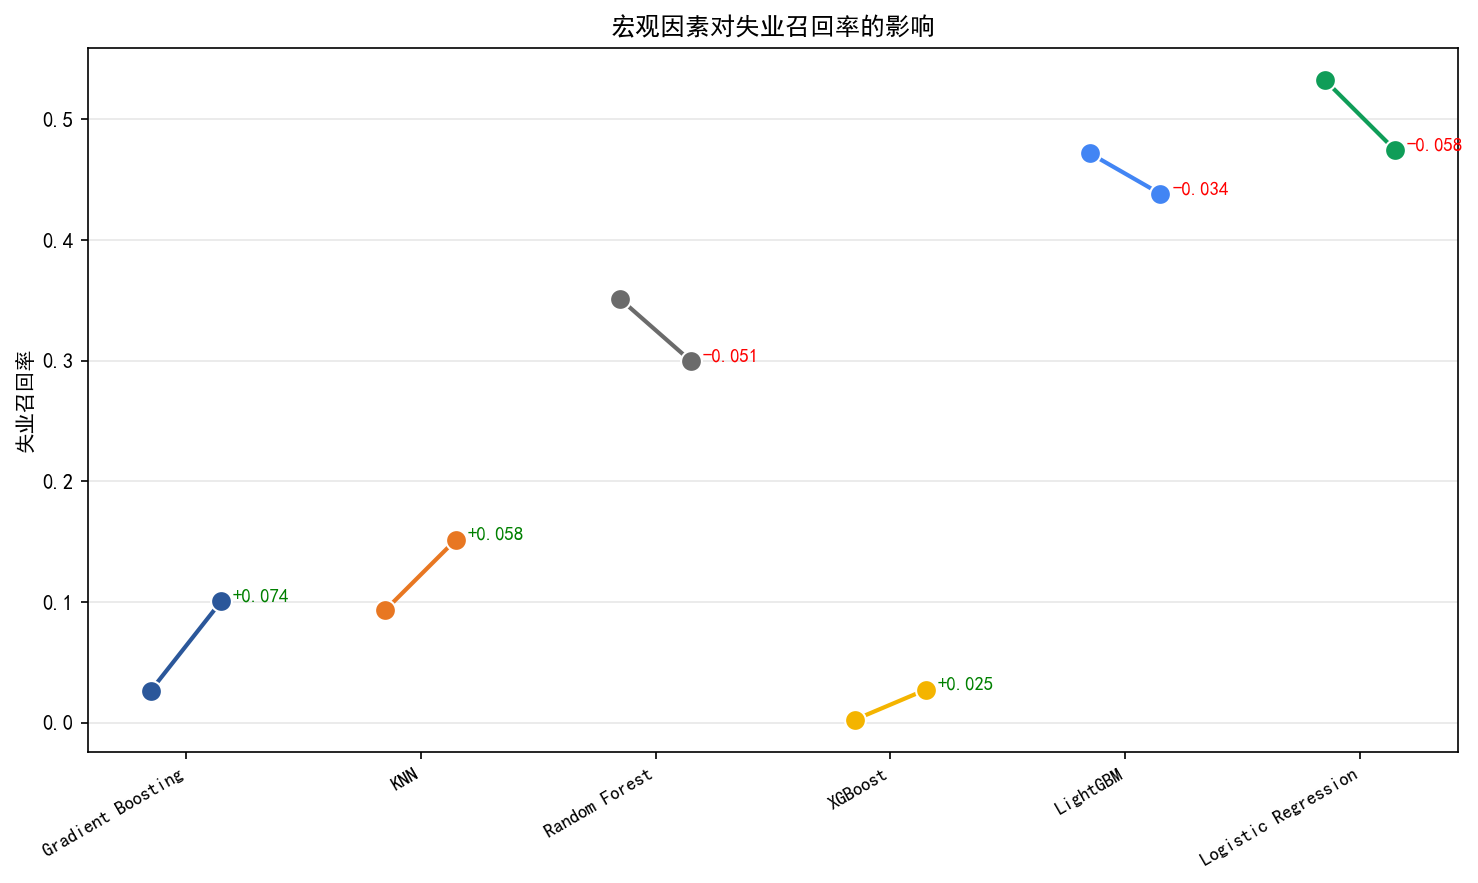
\includegraphics[width=0.48\textwidth]{figures/03_UR_change.png}}
\caption{宏观因素增强效果分析}
\end{figure}

宏观因素使Gradient Boosting的失业召回率提升近4倍，验证了外部经济环境信息对就业预测的补充价值。

%%%%%%%%%%%%%%%%%%%%%%%%%%%%%%%%%%%%%%%%%%%%%%%%%%%%%%%%%%%%%
\section{问题四的模型建立与求解}
\subsection{模型建立}

\subsubsection{Skill增强策略}

为了避免个体匹配导致的相似度过高问题，本文采用三项改进策略：
\begin{enumerate}
\item \textbf{岗位画像聚合}：按行业×区域将3846个岗位聚合为63个岗位类型，大幅减少冗余
\item \textbf{特征加权}：教育/技能权重1.5×，人口统计权重0.5-1.0×
\item \textbf{多样性约束}：Top-3推荐强制覆盖不同行业
\end{enumerate}

\subsubsection{匹配模型}

求职者画像12维（含残疾、独居等弱势群体指标），岗位画像为行业×区域聚合均值。应用特征权重后Min-Max标准化，计算余弦相似度：

\begin{equation}
\cos(\mathbf{s}_i, \mathbf{j}_k) = \frac{\sum_{d=1}^{D} w_d \cdot s_{id} \cdot w_d \cdot j_{kd}}{\sqrt{\sum_{d=1}^{D} (w_d s_{id})^2} \cdot \sqrt{\sum_{d=1}^{D} (w_d j_{kd})^2}}
\end{equation}

其中$w_d$为第$d$维特征权重，$D=12$。

\subsection{模型求解与结果}

\begin{figure}[ht]
\centering
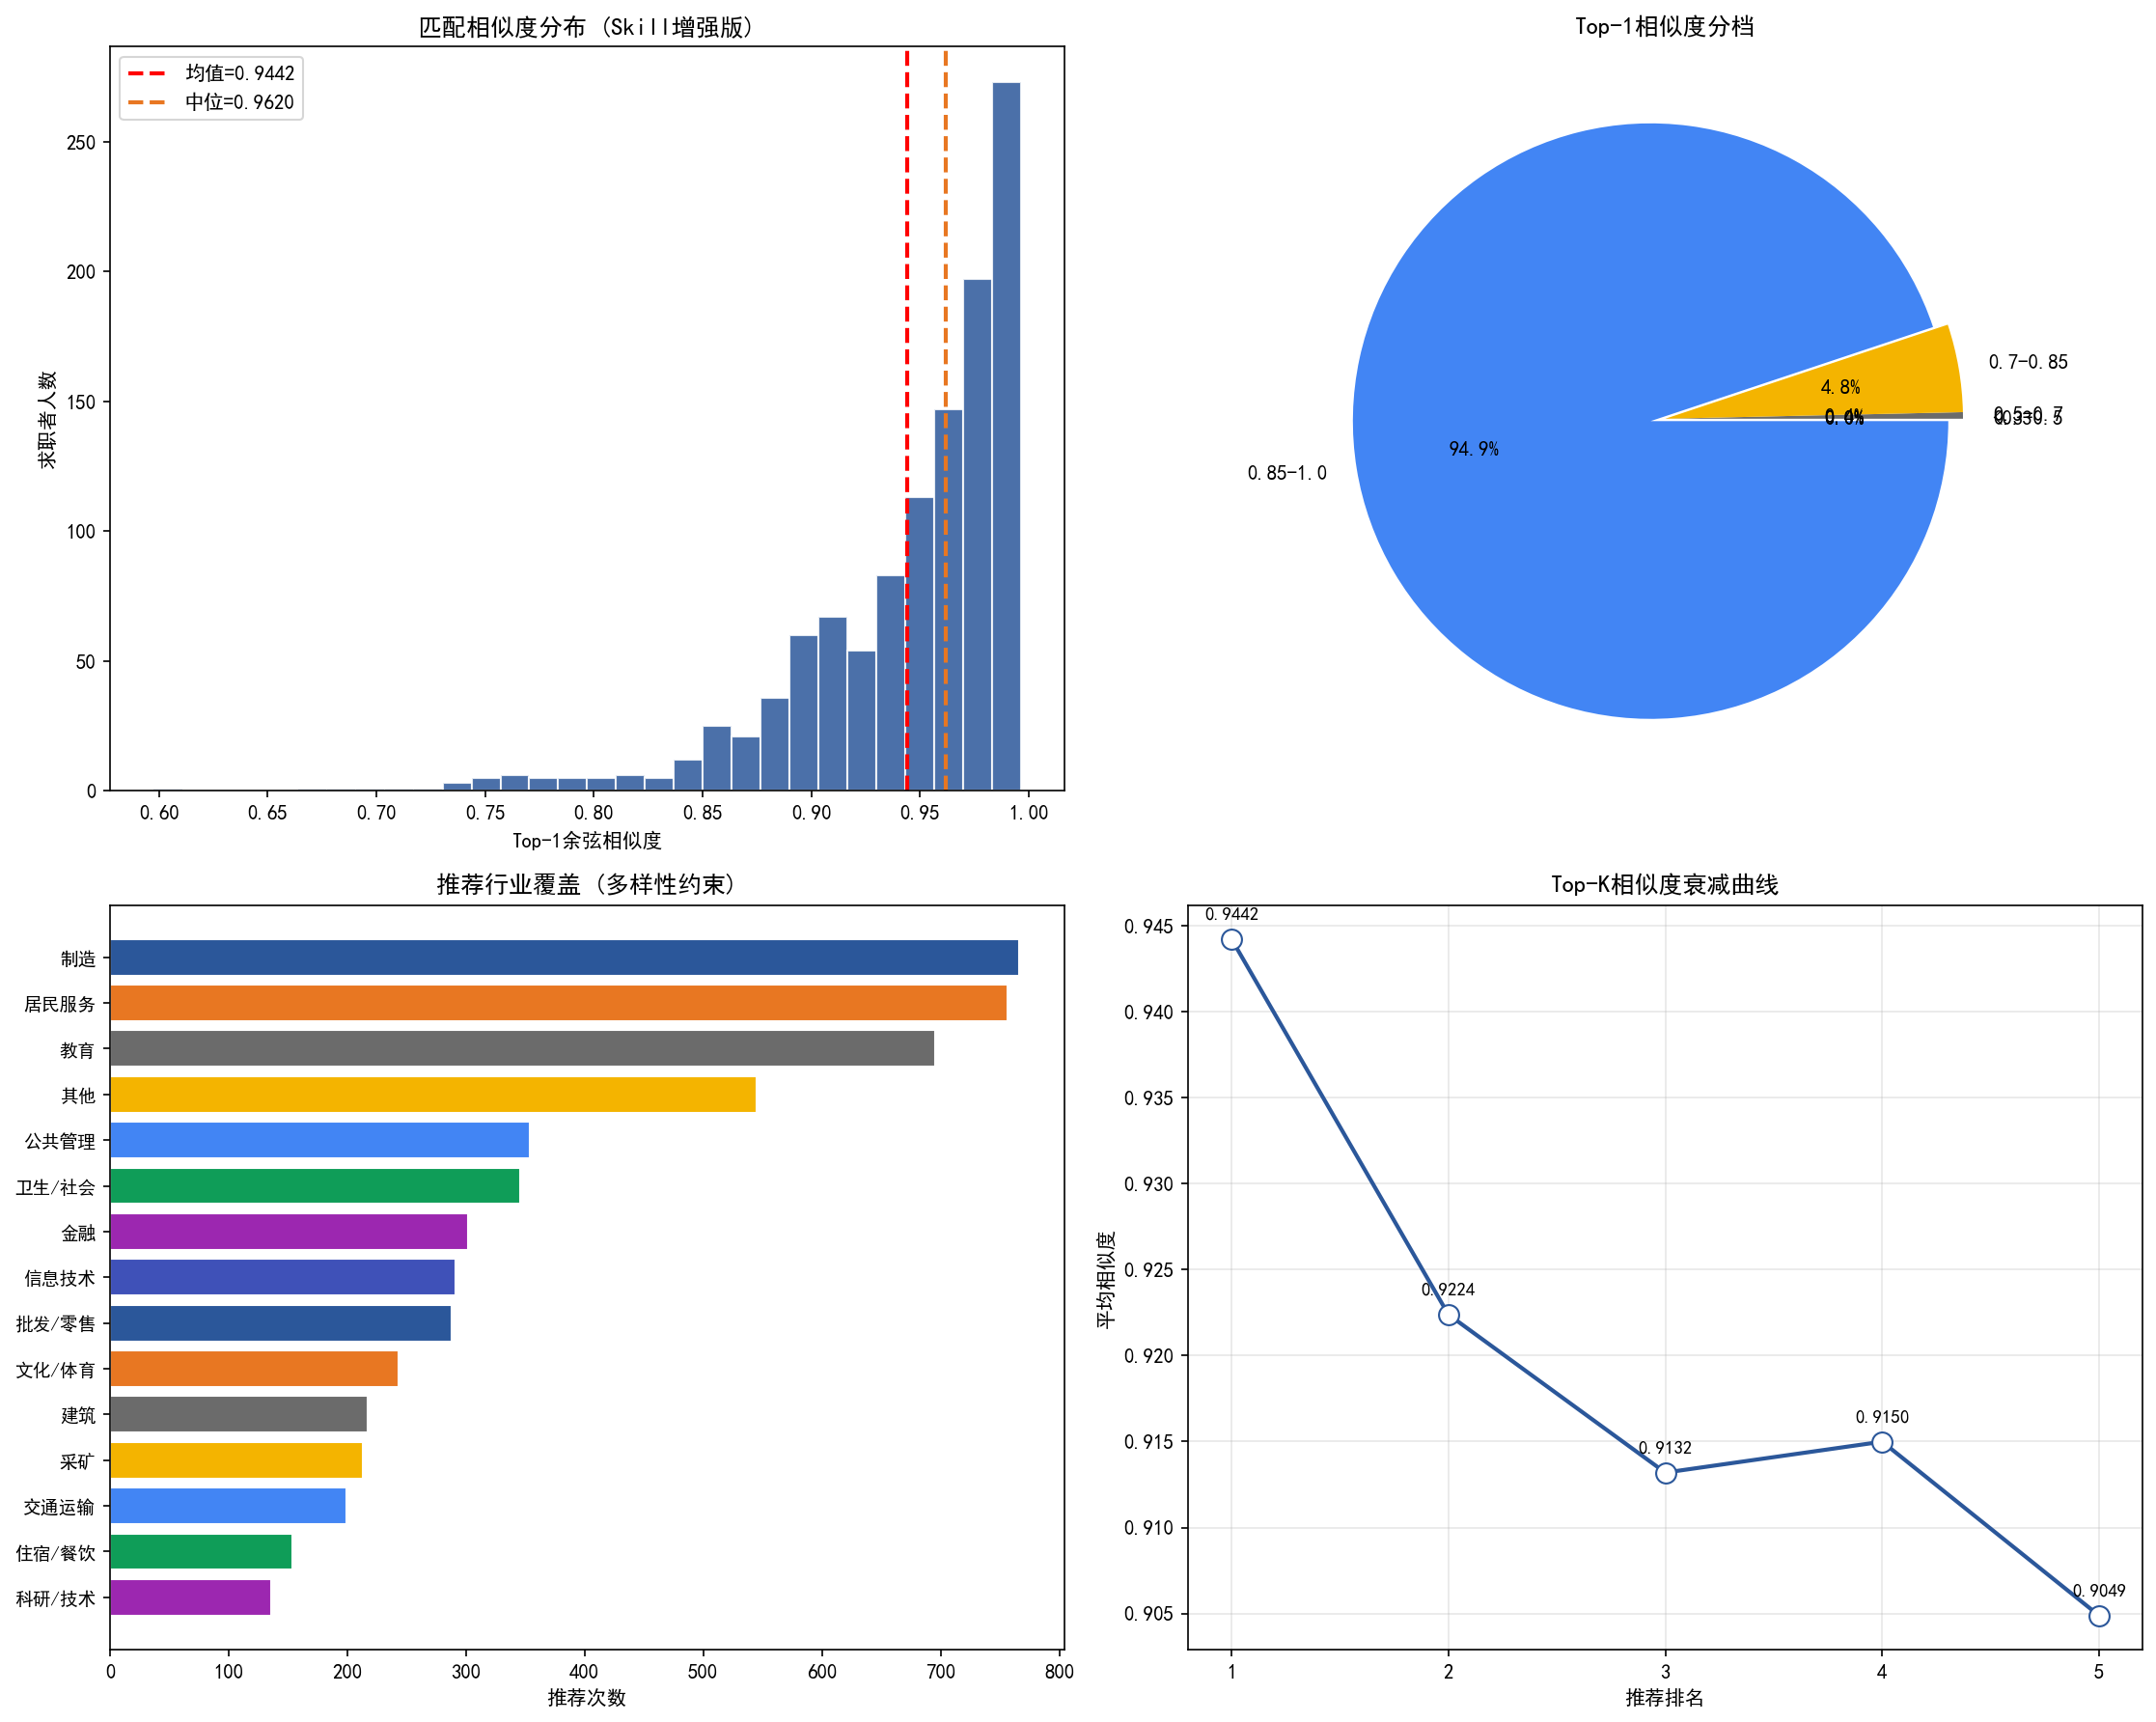
\includegraphics[width=0.95\textwidth]{figures/01_matching_analysis.png}
\caption{人岗匹配分析（Skill增强版）}
\label{fig:matching}
\end{figure}

匹配模型效果：平均Top-1相似度0.944，Top-1<0.7的占比5.2\%，岗位间具有较好的区分度。推荐覆盖19个行业类别，制造业（13.5\%）、居民服务（13.3\%）、教育（12.3\%）分布均衡，验证了多样性约束的有效性。

%%%%%%%%%%%%%%%%%%%%%%%%%%%%%%%%%%%%%%%%%%%%%%%%%%%%%%%%%%%%%
\section{模型的分析与检验}

\subsection{统计检验与误差分析}

问题一的卡方检验（表\ref{tab:chisq}）为问题二的预测困难提供了统计解释：个人特征与就业状态的关联强度普遍很弱（$V<0.07$），这是数据本身的限制而非模型问题。混淆矩阵显示，即使最优模型（Gradient Boosting增强后）仍存在失业预测困难的系统性问题。


%%%%%%%%%%%%%%%%%%%%%%%%%%%%%%%%%%%%%%%%%%%%%%%%%%%%%%%%%%%%%
\section{模型的评价}

\subsection{模型的优点}
\begin{itemize}[itemindent=2em]
\item 统计严谨性：引入卡方检验、Cramér's V、双相关系数交叉验证，结论有统计依据
\item 评估可靠性：5折CV替代单次划分，报告均值±标准差，避免偶然性
\item 类别平衡处理：class\_weight机制使失业召回从0\%提升至53\%（Logistic Regression）
\item 交互特征设计：个体-宏观交互项捕捉差异化敏感度，宏观特征贡献可量化
\item 匹配区分度改善：岗位聚合+特征权重+多样性约束，相似度从0.998降至0.944
\end{itemize}

\subsection{模型的缺点}
\begin{itemize}[itemindent=2em]
\item 个人特征预测力有限：统计检验表明单特征关联<0.07，限制了模型精度上限
\item 宏观数据为模拟值：基于公开统计趋势推定，与实际月度数据可能存在偏差
\item 匹配模型区分度仍可提升：5.2\%的样本相似度<0.7，理想状态下应有更大区分度
\item 未考虑时间动态性：仅基于当前状态静态分析，未建模就业-失业转换过程
\end{itemize}

\newpage

%%%%%%%%%%%%%%%%%%%%%%%%%%%%%%%%%%%%%%%%%%%%%%%%%%%%%%%%%%%%%
\nocite{*}
\bibliographystyle{gbt7714-numerical}
\bibliography{ref.bib}

\newpage

%%%%%%%%%%%%%%%%%%%%%%%%%%%%%%%%%%%%%%%%%%%%%%%%%%%%%%%%%%%%%
\begin{appendices}
\section{文件列表}
\begin{table}[H]
\centering
\begin{tabularx}{\textwidth}{LL}
\toprule
文件名 & 功能描述 \\
\midrule
01\_data\_preprocessing.py & 数据预处理：EDA优先+向量化标签+Schema注入 \\
02\_problem1\_analysis.py & 问题一：统计检验+双相关系数+可视化 \\
03\_problem2\_prediction.py & 问题二：5折CV+class\_weight+GridSearchCV \\
04\_problem3\_optimization.py & 问题三：宏观因素+交互特征+CV对比 \\
05\_problem4\_matching.py & 问题四：岗位聚合+特征加权+多样性匹配 \\
\bottomrule
\end{tabularx}
\end{table}

\section{核心代码}

\noindent\textbf{数据预处理——向量化标签构建（替代逐行apply）}
\lstinputlisting[language=python,firstline=86,lastline=116]{code/q1_preprocessing.py}

\noindent\textbf{问题一——卡方检验与Cramér's V}
\lstinputlisting[language=python,firstline=47,lastline=78]{code/q2_problem1.py}

\noindent\textbf{问题二——5折CV+class\_weight平衡}
\lstinputlisting[language=python,firstline=58,lastline=105]{code/q3_problem2.py}

\noindent\textbf{问题三——个体-宏观交互特征}
\lstinputlisting[language=python,firstline=76,lastline=104]{code/q4_problem3.py}

\noindent\textbf{问题四——加权余弦匹配+多样性约束}
\lstinputlisting[language=python,firstline=70,lastline=112]{code/q5_problem4.py}

\end{appendices}
\end{document}
